\documentclass{/home/daniel/GitHub/Cuadernos/Template}
\addbibresource{/home/daniel/GitHub/Cuadernos/Bibliografia.bib} % si quieres incluir la bibliografía

% Portada 
\title{\Huge \textbf{Introducción a las FPGAs}}
\author{\Large Daniel Vázquez Lago}

% Documento
\begin{document}
\pagenumbering{Roman}
\maketitle
\tableofcontents
\pagenumbering{arabic}
\setlength{\parskip}{2.2mm} % Cambia el espacio entre párrafos

\chapter{Sistemas FPGA}

\section{Concepctos básicos}

En esta sección introduciremos los conceptos básicos en diseño lógico. Presentaremos terminología importante usada en el resto del libro.

\subsection{Álgebra Booleana}

El \textbf{álgebra Booleana} representa las funciones lógicas de los circuitos digitales. Cualquier red de interruptores puede ser modelado por funciones Booleanas. Usamos el álgebra Booleana para describir \textbf{funciones lógicas combinacionales}. Las funciones lógicas básicamente permiten transformar una serie de \textit{inputs} (parámetros de entrada) en una serie de \textit{ouputs} (parámetros de salida). Sean $a$ y $b$ nuestras variables, definimos las siguientes funciones lógicas. Las funciones elementales (NOT, AND y OR) no tienen definición al ser precismante elementales, mientras que las no elementales las podemos definir a partir de las primeras. Sean $a$ y $b$ dos variables cualquiera, escribimos las funciones lógicas en la \cref{Tab:01-Funciones_Logicas}. 

\begin{table}[H] \centering
    \begin{tabular}{cccc} 
        \toprule 
        \textbf{Nombre} & \textbf{Símbolo } & \textbf{Definición} & \textbf{Ejemplo} \\ \midrule
        NOT & ' &  & (1)'=0 \ (0)'=1 \\
        AND  & $\cdot$ &  & 0$\cdot$0=1; 1$\cdot$0=0; 1$\cdot$1=1  \\
        NAND & |  & a | b = (a$\cdot$b)' & 0|0=1; 1|0 = 1; 1|1=0 \\
        OR  & $+$ &  & 0+0=0; 1+0 = 1; 1+1=1 \\
        NOR & NOR &  a NOR b = (a$+$b)' & 0 NOR 0 = 1; 1 NOR 0 = 0; 1 NOR 1 = 0 \\
        XOR & $\oplus$ & a $\oplus$ b = ab'+a'b & 0 $\oplus$ 0 = 0; 1 $\oplus$ 0 = 1; 1 $\oplus$ 1 = 0\\
        XNOR & XNOR & a XNOR b = (a $\oplus$ b)'  & 0 XNOR 0 = 1; 1 XNOR 0 = 0; \\ \bottomrule
    \end{tabular} 
    \caption{}
    \label{Tab:01-Funciones_Logicas}
\end{table}

Lógicamente, como toda álgebra, el álgebra de Boole sigue ciertas reglas de aritmética básicas, tales como: 

\begin{itemize}
    \item \textbf{Ley asociativa:} a + (b+c) = (a+b)+c; a $\cdot$ (b$\cdot$c) = (a $\cdot$ b )$\cdot$c.
    \item \textbf{Ley distributiva:} (a+b)' = a' $\cdot$ b'; (a$\cdot$b)' = a' $+$ b'
\end{itemize}

\subsection{Símobolos lógicos y eléctricos}

Los símbolos eléctricos más usados son: 

\begin{figure}[H] \centering
\begin{circuitikz}
  % NMOS
  \draw (0,0) node[nmos] (N) {};
  \node[below=0.2cm of N] {n-mosfet};

  % PMOS, desplazado
  \draw (3,0) node[pmos] (P) {};
  \node[below=0.2cm of P] {p-mosfet};

  % Dibuja una resistencia con etiquetas
  \draw (4.5,0) to[R, l=$ $] (7,0);
  
  \node (R) at (6,0) {};
  \node[below=0.8cm of R] {Resistencia};

  % Dibuja un capacitor 
  \draw (8,0) to[C, l=$ $] (10,0);
  \node (C) at (9,0) {};
  \node[below=0.8cm of C] {Capacitor};
\end{circuitikz}
\caption{Símbolos para esquemas eléctricos.}
\end{figure}

Mientras que los símbolos en circuitos lógicos son: 

\begin{figure}[H] \centering
\begin{tikzpicture}[scale=10]

  % Inverter
  \node[not gate US, draw, logic gate inputs=nn] (inv) {};
  \node[below=0.2cm of inv] {NOT};

  % NAND
  \node[nand gate US, draw, logic gate inputs=nn, right=1.5cm of inv] (nand) {};
  \node[below=0.2cm of nand] {NAND};

  % NOR
  \node[nor gate US, draw, logic gate inputs=nn, right=1.5cm of nand] (nor) {};
  \node[below=0.2cm of nor] {NOR};

  % AND
  \node[and gate US, draw, logic gate inputs=nn, below=1.5cm of inv, xshift=0.9 cm]  (and) {};
  \node[below=0.2cm of and] {AND};

  % OR
  \node[or gate US, draw, logic gate inputs=nn, right=1.5cm of and] (or) {};m.
  \node[below=0.2cm of or] {OR};

  % XOR
  \node[xor gate US, draw, logic gate inputs=nn, below=1.5cm of and] (xor) {};
  \node[below=0.2cm of xor] {XOR};

  % XNOR
  \node[xnor gate US, draw, logic gate inputs=nn, right=1.5cm of xor] (xnor) {};
  \node[below=0.2cm of xnor] {XNOR};

\end{tikzpicture}
\caption{Símbolos para esquemas lógicos.}
\end{figure}

\section{Diseño digital y FPGAs}

\subsection{El papel de las FPGAs}

Los \textbf{FPGAs} (\textit{Field Programmable Gate Arrays}, en español matriz de puertas lógicas programable en campo) llenan una necesidad existente en el diseño de sistemas digitales, complementario al rol que juegan los microprocesadores. Los microprocesadores pueden ser usados en una cantidad de entornos enorme, pero porque ellos confian en el software para implementar funciones, aunque son generalmente más lentos y consumen más potencia que los chips diseñados con un único propósito (\textit{customizados}). De manera similar, los FPGAS no son chips a medida, por lo que no son tan buenos en funciones particulares. Sin embargo poseen grandes ventajas: 

\begin{itemize}
    \item No tienes porque esperar a acabar el diseño para obtener un chip funcional: el diseño puede ser programado y testeado inmediantemente. 
    \item Son excelentes prototipos. Cuando un FPGA tiene un diseño final, crear un producto o un chip customizado suele ser mucho más fácil.
    \item El mismo FPGA puede ser usado con diferentes diseños. 
\end{itemize}

El área ocupada por las FPGA ha crecido enormemente en los últimos veinte años desde su introducción. Los \textbf{dispositivos de lógica programable PLD} (\textit{Programmable Logic Devices}) estaban en el mercado desde principios de la década de 1970. Estos dispositivos utilizaban estructuras de lógica de dos niveles para implementar la lógica programada. El primer nivel de lógica, el plano AND, generalmente era fijo, mientras que el segundo nivel, conocido como el plano OR, era programable. Los PLD se programaban, en general, mediante antifuses, que se activaban aplicando altos voltajes para establecer las conexiones.

Se utilizaban con mayor frecuencia como \textbf{lógica de enlace } (\textit{glue logic}): lógica necesaria para interconectar los componentes principales del sistema. A menudo se empleaban en prototipos porque podían programarse e insertarse en una placa en cuestión de minutos, pero no siempre llegaban a formar parte del producto final. Los dispositivos de lógica programable no solían considerarse componentes principales de los sistemas en los que se utilizaban. A medida que los sistemas digitales se hicieron más complejos, se necesitaba lógica programable de mayor densidad, y se hicieron evidentes las limitaciones de la lógica de dos niveles de los PLD. La lógica de dos niveles es útil para funciones lógicas relativamente pequeñas, pero con el aumento del nivel de integración, las estructuras de dos niveles se volvieron demasiado ineficientes.

Las FPGA proporcionaron lógica programable usando lógica multinivel de profundidad arbitraria. Utilizaban tanto elementos de lógica programable como interconexiones programables para construir funciones lógicas multinivel. 

A Ross Freeman se le atribuye generalmente la invención de la FPGA. Su FPGA incluía tanto elementos lógicos programables como una estructura de interconexión programable. Su FPGA también se programaba usando memoria SRAM, no antifuses. Esto permitía fabricar la FPGA utilizando procesos estándar de fabricación VLSI, lo que reducía los costos y ofrecía más opciones de manufactura. También permitía que la FPGA se reprogramara mientras estaba en el circuito; esta era una característica particularmente interesante dado que la memoria flash aún no se utilizaba de forma generalizada.

Xilinx y Altera comercializaron las primeras FPGA basadas en SRAM. Una arquitectura alternativa fue introducida por Actel, que empleaba una arquitectura de antifuses. Esta arquitectura no era reprogramable en el campo, lo que se consideraba una ventaja en situaciones que no requerían reconfiguración. Las FPGA de Actel utilizaban una estructura lógica basada en multiplexores organizada en torno a canales de cableado

Durante muchos años las FPGAs han sido vistos como dispositivos de lógica de enlace y como dispositivos para generar prototipos. Hoy en día son usados en todo tipo de sistemas digitales, especialmente en los siguientes campos:
\begin{itemize}
    \item En sistemas de telecomunicaciones extremadamente rápidos.
    \item Como aceleradores de video en grabadoras de video personales.
\end{itemize}

\subsection{Tipos de FPGA}

Pese a qeu hemos hablado de ellos, aún no hemos definido que es un FPGA. Una buena definición podría ser directamente enumerar las características de los PLDs  y los chips customizado, tales como:

\begin{itemize}
    \item Son partes estándar. No estan diseñadas con un propósito particular, pero si son programadas para un propósito particular.
    \item Implementan lógica multi-nivel. Los bloques lógicos dentro de las FPGAs pueden funcioanr como redes de una profundidad arbitaria. Los PLDs por otro lado solo usan dos niveles lógicos: NAND/NOR, lo que limita el tipo de funciones que se pueden implementar eficientemente, pues cualquier función booleana compleja debe transformarse a una forma de solo dos niveles, lo que puede requerir muchas puertas y dificultar el diseño. 
\end{itemize}
Dad que los FPGAs implementan lógica multinivel, son  a la vez bloques lógicos programables y interconexiones programables. 

Para que una FPGA funcione como un circuito digital personalizado, no basta con tener bloques lógicos programables (por ejemplo, LUTs, flip-flops, multiplexores configurables, etc.); también se necesita un sistema que permita conectarlos de cualquier forma necesaria, lo cual se logra con las interconexiones programables.

\begin{itemize}
    \item Los bloques lógicos programables implementan las operaciones lógicas básicas y permiten que el usuario defina qué función booleana realiza cada bloque.

    \item Las interconexiones programables son una red de caminos (switches, multiplexores, etc.) que permiten unir las entradas y salidas de los bloques lógicos según el diseño que el usuario desee. Gracias a ellas, se puede construir cualquier topología de circuito, desde simples puertas combinacionales hasta máquinas de estado complejas.
\end{itemize}
La combinación de bloques lógicos programables y interconexiones programables se llama \textit{fabric} o \textbf{malla} porque posee una estructura regular que puede ser utilizada eficientemente por las herramientas de diseño que asignan la lógica deseada a la FPGA.

Se utilizan diversas tecnologías para programar las FPGA. Algunas FPGA se programan de forma permanente; otras pueden reprogramarse. Las FPGA reprogramables también se conocen como dispositivos reconfigurables. Las FPGA reconfigurables suelen ser preferidas en la construcción de prototipos porque no es necesario desechar el dispositivo cada vez que se realiza un cambio. Los sistemas reconfigurables también pueden reprogramarse dinámicamente durante el funcionamiento del sistema. Esto permite que un mismo hardware desempeñe varias funciones diferentes. Por supuesto, esas funciones no pueden ejecutarse al mismo tiempo, pero la reconfigurabilidad puede ser muy útil cuando un sistema opera en diferentes modos. Por ejemplo, la pantalla del ordenador Radius funcionaba tanto en modo horizontal (paisaje) como en modo vertical (retrato). Cuando el usuario rotaba la pantalla, un interruptor de mercurio provocaba que la FPGA que gestionaba la pantalla se reprogramara para el nuevo modo.

%El FPGA guarda un diseño como un “mapa” de cómo deben estar los switches, y al aplicarlo físicamente, transforma el chip genérico en un circuito específico que implementa tu lógica de manera real y operativa. Un FPGA no es solo una red de switches y LUTs: es un sistema completo de bloques lógicos, memorias, DSPs, interconexiones, interfaces de E/S y circuitería de gestión, todo integrable y configurable para implementar desde una simple puerta lógica hasta sistemas complejos como microcontroladores, procesadores, o procesadores de señal digital.

\section{Lógica Combinacional y secuencial}
Por un lado la \textbf{,ógica combinacional:}
\begin{itemize}
  \item La salida depende únicamente de las entradas actuales.
  \item No existe memoria: el circuito no recuerda estados pasados.
  \item Ejemplos: puertas lógicas, multiplexores, decodificadores, sumadores combinacionales.
\end{itemize}

\[
\text{Salida}(t) = f(\text{Entradas}(t))
\]
por otro lado la \textbf{lógica secuencial:}
\begin{itemize}
  \item La salida depende de las entradas actuales y del estado anterior del sistema.
  \item Utiliza elementos de almacenamiento como flip-flops o latches.
  \item Ejemplos: contadores, registros, máquinas de estados, sistemas de control.
\end{itemize}

\[
\text{Estado}(t+1) = f(\text{Entradas}(t), \text{Estado}(t))
\]
\[
\text{Salida}(t) = g(\text{Entradas}(t), \text{Estado}(t))
\]

La diferncia esencial es entonces que la lógica combinacional no tiene memoria; la lógica secuencial sí, permitiendo que el comportamiento del circuito dependa del tiempo y del historial de entradas.

La \textbf{lógica combinacional} se utiliza para operaciones que requieren procesar las entradas únicamente en el momento actual, sin necesidad de memoria. Es ideal para construir sumadores, restadores, multiplexores, comparadores, decodificadores y en general cualquier circuito que realice una operación aritmética o lógica de manera instantánea. Por ejemplo, se usa para procesar datos en una unidad aritmético-lógica (ALU), decidir rutas en un multiplexor o traducir direcciones en un decodificador. La \textbf{lógica secuencial} se emplea cuando es necesario que el circuito recuerde información, es decir, cuando su comportamiento depende del historial de entradas (los estados anteriores). Se utiliza en contadores para llevar la cuenta de eventos, registros para almacenar datos temporalmente, máquinas de estados para implementar protocolos de comunicación, controladores secuenciales como los de microprocesadores, y pipelines para procesar varias etapas de datos de manera sincronizada. Ejemplos de su uso incluyen cronómetros digitales, controladores de robots, memorias intermedias FIFO y la ejecución paso a paso de instrucciones en un procesador.



 \chapter{Tecnología VLSI}

Mientras que el diseño tradicional de los sistemas VLSI (Very Large Scale Integration) tiene sus días contados, el diseño a través de las FPGAs está en auge. Sin embargo, los diseñadores de grandes sistemas FPGA necesitan entender los fundamentos de VLSI para sacar el máximo rendimiento a los FPGAs. La arquitectura de los FPGAs está determinada completamente por las restricciones que imponen los VLSI: estructuras de elementos lógicos, estructuras de interconexión programables, redes de interconexión, configuración, distribución de pines. Entender como las características de los dispositivos VLSI afectan a las estructura FPGA pemitirá al diseñador entender cuales son las mayores ventajas de los FPGAs y minimizar la influencia de sus limitaciones. 

Tomemos por ejemplo las redes de interconexión en FPGAs. La mayor parte de los FPGAs modernos proveen a los diseñadores de diferentes tipos de conexiones: locales, globales... ¿Por qué existen tantos tipos de conexiones? Porque las conexiones son cada vez más dificiles de manejar, debido al aumento de longitud. Entender como funcionan estas diferentes tipos de conexión ayudarán al diseñador a elegir que tipo particular de conexión lógica usar, disminuyendo costes y/o aumentando la eficiencia. 

En este capítulo nos centtaremos en entender los VLSI: fabricación, circuiteria, interconexiones... 

\section{Procesos de manufactura}

\lipsum[1]

\lipsum[1]

\section{Características de los transistores}

\lipsum[1]

\lipsum[1]

\section{Puertas Lógicas CMOS}

En esta sección vamos aprender sobre la lógica CMOS, el elemento baśico en el diseño lógico. Para entender el funcionaiento básico de las puertas lógicas, también debeos entender las características básicas de los transistores. Primero introduciremos el diseño básico de las puertas, dado que las puertas más simples pueden ser entendidas pensando en los transistores como interruptores. 

\subsection{Puertas estáticas complementarias}

Consideremos por el momento los transistores como interruptores perfectos. La condición de encendido será diferente cuando consideremos un transistor tipo P y tipo N: un tipo N está encendido cuando el voltaje de puerta es positivo respecto el sustrato, mientras que en el tipo P estará encendido cuando sea negativo. 

La estructura básica de una puerta CMOS está basa en las \textbf{puertas estáticas complementarias}. ¿Por qué se llaman así? El término estático viene de que la salida se mantiene estable (0 o 1) mientras la entrada no cambie. No requiere un reloj ni refresco para mantener su valor. El término complementario viene de que la red NMOS y la red PMOS son complementarias entre sí, i.e. que alguna de las salidas de los transistores NMOS y PMOS debe estar conectada a la salida en todo momento. 

Está divida en la \textbf{\textit{red pullup}} y \textbf{\textit{red pulldown}}, hechas de transistores tipo-p y tipo-n. La salida de la puerta puede ser conectadas al potencial $V_{DD}$ (\textit{Voltaje Drain to Drain}, normalmente 5 V o el 1 lógico) o al potencial $V_{SS}$ (\textit{Voltaje Source to Source}, normalmente 0 V o el 0 lógico). Las dos redes deben ser complementarias para que podamos obtener una salida no indeterminada, y para que además no exista ningún caso de que la salida esté conectada a ambas a la vez. Veamos algunos ejemplos. 

\begin{Ejemplo}
    Ejemplo 2.1: inversor
\end{Ejemplo}

\begin{minipage}{0.65\linewidth}
El esquema para el inversor es extremadamente sencillo pero extremadamente ilustrativo. En este caso la entrada $a$, que puede tener un valor de 1 (volatje 5 V, +) o un valor de 0 (voltaje 0 V, triangular) se conecta a la base del transistor NMOS y PMOS. Como hemos dicho, estos funcionan como interruptores perfectos, pero complementarios. El detector NMOS (abajo) dejará estará encedido (deja pasar corriente) cuando reciba un voltaje positivo (respecto la entrada), es decir, cuando reciba un \textit{input} 1, mientras que el PMOS (arriba) cuando recibe un voltaje negativo (\textit{input} 0). Dado que el NMos está conectado con el $V_{SS}$ (\textit{output} 0), cuando reciba el 1 saldrá el \textit{output} 0, e viceversa cuando se conecte el PMos. En la figura \cref{Fig:02-InversorV} vemos el voltaje de salida frente al de entrada.
\end{minipage}
\hfill
\begin{minipage}{0.32\linewidth} \centering
    \includegraphics[width=1\linewidth]{Imagenes/02/02-InversorDiseñado.png}
    \captionof{figure}{Esquema del inversor con nMOS y pMOS.}
    \label{Fig:02-Inversora}
\end{minipage}


\begin{figure}[H] \centering
\begin{tikzpicture}
\begin{axis}[
    xlabel={$V_{in}$ [V]},
    ylabel={$V_{out}$ [V]},
    grid=both,
    title={Respuesta del inversor},
    legend pos=south west,
    width=12cm,
    height=8cm,
]
\addplot[
    color=blue,
    mark=*,
] table [x=V2, y={V(n002)}, col sep=space] {Imagenes/02/Inversor_V.txt};
\addlegendentry{$V_{in}$ vs $V_{out}$}
\end{axis}
\end{tikzpicture}
\caption{Representación gráfica del voltaje de salida para \cref{Fig:02-Inversora} frente al voltaje de entrada, donde vemos claramente que con el 0 lógico de entrada (0 V) tenemos el 1 de salida (5 V); y que con el 1 de entrada (5 V) tenemos el 0 de salida (0 V).}
\label{Fig:02-InversorV}
\end{figure}



\subsection{Retardo de la Puerta Lógica}

El \textbf{retardo} es una de las características más importantes de las puertas lógicas, y es el tiempo que tarda una puerta en cambiar su salida del valor lógico 0 a 1 o viceversa. Sin embargo, para entenderl obien tenemos que definir correctamente que valores de voltaje son el 0 y el 1, ya que aunque hallamos trabajado con 0 V y 5 V respectivamente, en realidad habrá un cierto margen, un cierto rango que se considerá un 0 y un 1. Esto está definido por dos voltajes $V_H$ y $V_L$ (de \textit{Hight Voltaje} y \textit{Lower Voltaje}) que nos dan el voltaje inferior para el 1 lógico (5 V) y el valor superior del 0 lógico (0 V).

Cuando entra un voltaje entre $V_H$ y $V_{DD}$ estamos efectivamente en el 1 lógico, mientras que cuando estamos en el $V_L$ y $V_{SS}$ en el 0 lógico. La definición de los valores $V_L$ y $V_H$ dependen del detector. En muchos casos denotamos por $V_{IH}$ y $V_{IL}$ cuando se tratan de los valores de entradas (\textit{inputs}). 

El retardo que tenga una puerta lógica se puede modelar en el esquema con una resistencia y un condensador en serie (un RC) como en la \cref{Fig:02-Inversora_RC}, aunque en la realidad tenga un forma mucho más compleja.

\begin{figure}[H] \centering
    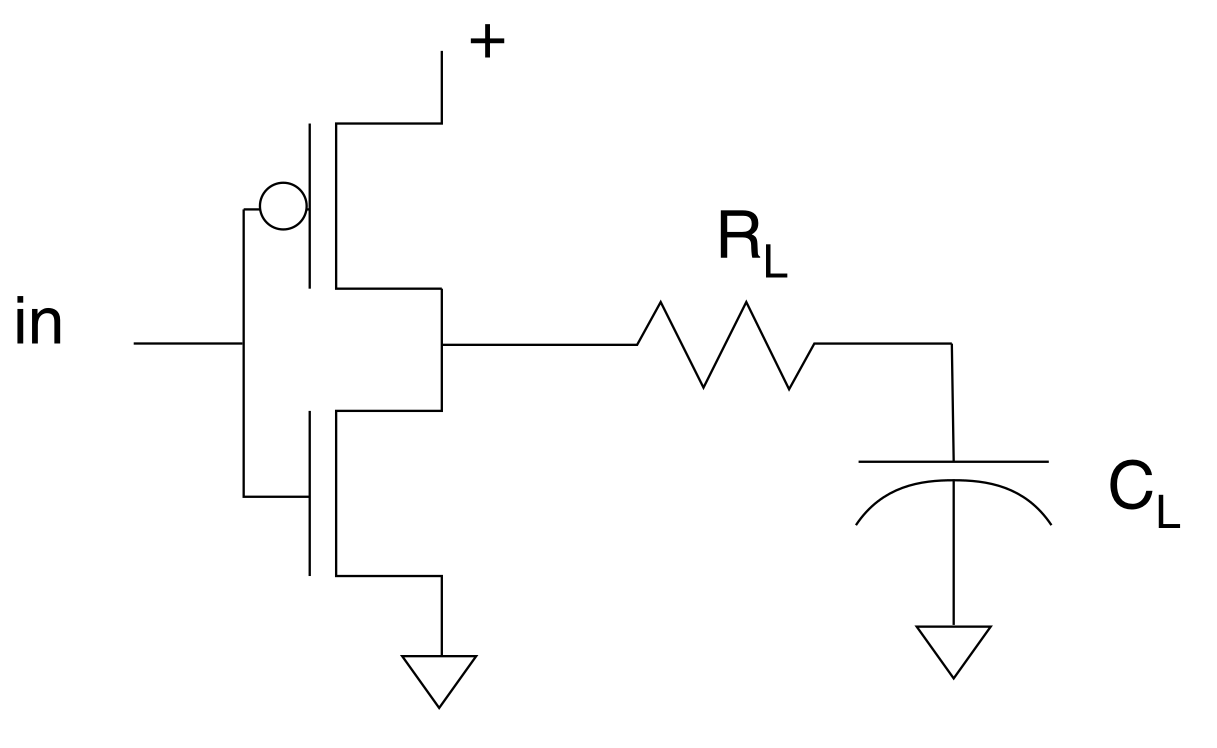
\includegraphics[width=0.7\linewidth]{Imagenes/02/02-Inversor_2.png}    
    \caption{modelización del retardo de puerta lógica inversora.}
    \label{Fig:02-Inversora_RC}
\end{figure}


El \textbf{modelo tau ($\boldsymbol{\tau}$)} nos da un valor para el retardo. Este modelo reduce el retardo de la puerta a un RC de tiempo constante $\tau$ para ambos modos. Que un transistor este modelado por una resistencia $R_n$ puede sonar un poco raro, y más cuando el transitor no obedece una ley lineal de entrada-salida (ley de Ohm). Por ello seleccionar una resistencia puede ser un poco complicado. Lo que se hace normalmente es asumir que la resistencia es un promedio del voltaje en saturacion y en el comporamiento lineal: 

\begin{equation}
    R_n = \frac{1}{2} \parentesis{\frac{V_{sat}}{I_{sat}}+\frac{V_{lin}}{I_{lin}}}
\end{equation}
Los valores de voltaje e intensidad de saturación y lineal dependerán del transistor. Además tenemos la \textit{resistencia de carga} (\textit{load resistance}), que es la resistencia efectiva que se conecta a la salida de un circuito. Es el elemento resistivo que determina cuánta corriente debe entregar el circuito para mantener un determinado voltaje en la salida.Esta resistencia de carga suele está conectada en serie con la resistencia $R_n$, por lo que la resistencia efectiva es: 

\begin{equation}
    R_{eff} = R_n + R_L
\end{equation} 
El tiempo de retardo vendrá dado por: 

\begin{equation}
    \tau \propto (R_n + R_L) C_L
\end{equation}
Otro modelo es el \textbf{modelo para una fuente de corriente}, el cual se suele usar en estudios de potencia-retardo. Si asumimos que el transistor actúa como una fuente de corriente cuyo $V_{gs}=V_g-V_s$\footnote{El $V_{gs}$ es el que controla que el canal este formado, por lo que si es menor que el umbral el transistor no estará encendido y si supera el umbral en transistor estará encendido.} está siempre al máximo valor, entonces el tiempo que tarda en decaer viene dado por 

\begin{equation}
    t_f = \frac{C_L (V_{DD}-V_{SS})}{I_d}
\end{equation}
Otro modelo es el \textbf{modelo ajustado}, que directamente lo que hace es medir experimentalmente las características del sistema y ajustarlas con una función que sea capaz de reproducirla. Suele ser usada en programas que analizan un gran número de puertas. 

Este análisis con RC nos arroja información sobre el retardo temporal. En primer lugar, que los retardos de 0 a 1 y de 1 a 0 serán diferentes (el 0 a 1 será más rápido, entorno a la mitad o un ternio de 1 a 0) debido a la diferencia del ratio de las resistencias efectivas. 

\subsection{Consumo de potencia}

En consumo de potencia es un punto importante cuando hablamos sobretodo de dispositivos en la vida real. El consumo en los circuitos CMOS depende directamente de la frecuencia en la que operen los aparatos, del tamaño de los transistores (sobretodo aquellos que tengan mayor influencia en la capacidad), así como de la diferencia de los voltajes $V_{DD}$ y $V_{SS}$ en los que opere el circuito, tal que la potencia $P$ es

\begin{equation}
    P = f C_L (V_{DD}-V_{SS})^2
\end{equation}
siendo $f$ la \textit{frecuencia de reloj} y $C_L$ la capacidad del sistema. En muchas ocasiones hablamos de la \textit{speed-power} a la périda de energía que ocurre en una sola transición, definida como el producto $SP=CV^2$. Como podemos ver, las pérdidas de energía se reducen cuando disminuimos el voltaje al que operamos, por eso se busca usar puertas lógicas en paralelo. Reducir el voltaje hace más lentos los transistores, por lo que tienes que disminuir la frecuencia si quieres bajar el voltaje. Ahoran, si necesitas procesar la misma cantidad de datos por segundo, agregas más unidades lógicas en paralelo, cada una trabajando más despacio (menor frecuencia) pero todas colaborando para mantener el rendimiento global. A esta técnica se le llama \textbf{escalado de voltaje}.

\subsection{Manejando grandes cargas}

\subsection{Puertas de baja potencia}

\subsection{\textit{Switch Logic}}


El símbolo mostrado en la  \cref{Fig:02-switch} representa un transistor de transmisión controlado por una señal de reloj o fase. También se le llama switch controlado o interruptor de transmisión.

La señal a en la parte superior indica la señal de control: cuando a está activa, el interruptor se cierra y conecta las dos líneas horizontales. La señal a' (a prima) representa la fase complementaria: a' es simplemente la inversión de a, aunque en el símbolo no siempre se conecta explícitamente; a menudo solo se indica que este interruptor trabaja con fases alternas.

Cuando a está en nivel alto (a=1), el interruptor cierra el contacto, permitiendo que la señal de la línea izquierda pase a la derecha y viceversa. Es decir, el interruptor está conduciendo. Cuando a está en nivel bajo (a=0), el interruptor se abre, aislando eléctricamente ambos lados; las señales no pueden pasar.

\begin{figure}[H] \centering
    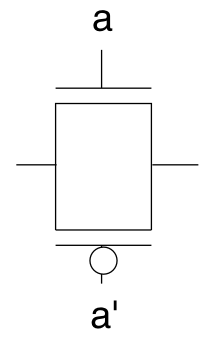
\includegraphics[width=0.3\linewidth]{Imagenes/02/02-Switch}
    \caption{Puerta de trasmisión complementaria.}
    \label{Fig:02-switch}
\end{figure}

¿Por  que hay dos transistores, un n-mos y un p-mos? Porque la conducción de n-mos depende de si el valor de entrada es 0 o 1, ya qeu conduce bien para 0 pero mal para 1. Con a y a' esto se soluciona: cuando a=1, el nMOS se enciende y a'=0, el pMOS también se enciende, ambos conducen y el paso es limpio en todo el rango de tensión. Cuando a=0, el nMOS se apaga y a'=1, el pMOS se apaga, ambos desconectados y el paso cortado.

\section{Cables}

\subsection{Estrcutra de los cables}

\subsection{Modelos de cables}


\section{Registros y RAM}

La memoria en sus difernetes formas es muy importante en el diseño digital y particularmente interesante en los FPGAs. En este sección vamos a hablar de los registros -elementos de memoria diseñados para hacer operaciones de reloj- y el acceso a memoria.  

En este contexto, un \textbf{reloj} es una señal eléctrica periódica que alterna entre niveles alto y bajo.  Cada transición de la señal de reloj se llama \textbf{flanco}. El \textbf{tiempo de setup} (setup time) es el tiempo mínimo que la señal de datos (D) debe estar estable antes del flanco activo del reloj (por ejemplo, el flanco de subida) para que el registro pueda capturarla correctamente. El \textbf{tiempo de hold} (hold time) es el tiempo mínimo que la señal de datos debe permanecer estable después del flanco activo del reloj, para asegurar que el registro complete la captura del dato.

Los \textbf{\textit{latches}} (biestable) son elementos de almacenamiento que guardan un bit y cuya salida sigue la entrada mientras la señal de habilitación está activa (nivel alto o bajo, según el diseño). Por eso se dice que son transparentes: mientras la habilitación esté activa, cualquier cambio en la entrada se refleja inmediatamente en la salida. Cuando la habilitación deja de estar activa, el latch mantiene el último valor capturado.

Los \textbf{flip-flop} también almacenan un bit, pero su salida solo se actualiza en el instante de un flanco del reloj (subida o bajada). Esto significa que los datos se capturan solo en un momento preciso definido por el reloj, no mientras un nivel esté activo. Por eso son la base de los registros sincrónicos en circuitos digitales.

\subsection{Estrucutra de los registros}

Construir una máquina secuencial requiere \textbf{registros} que lean un valor, lo guarden durante un tiempo, y que luego puedan escribir  el valor guardado en algún sitio, incluso si el valor de entrada cambia  para asegurar que la máquina secuencial opere correctamente paso a paso. Es decir, una vez que el registro captura un dato, ese dato queda “congelado” dentro del registro hasta que el reloj indique que debe capturar un nuevo valor. 


En los circuitos CMOS, la memoria de un registro se forma por algún tipo de capacitancia o mediante retroalimentación positiva de energía desde la fuente de alimentación. El acceso a la memoria interna se controla mediante la entrada de reloj: el elemento de memoria lee el valor de su entrada de datos cuando el reloj lo indica y almacena ese valor en su memoria. La salida refleja el valor almacenado, probablemente después de algún retardo. Los registros difieren en muchos aspectos clave:

\begin{itemize}
    \item La forma de la señal de reloj que imprime el valor de entrada en el registro. 
    \item Como el comportamiento de la información sobre la señal de lectrua de un reloj afecta al valor guardado. Ejemplo: Supón que el registro necesita un setup de 5 ns y un hold de 1 ns. Si el dato cambia 1 ns antes del flanco, se violó el setup, y entonces el valor almacenado puede ser incorrecto. Si el dato cambia 0.5 ns después del flanco, entonces se violó el hold, y también puede capturarse un valor erróneo.
    \item Cuando el valor guardado es presentado como un valor de salida . 
    \item Si alguna vez existe un camino combinacional desde la entrada hasta la salida. Se refiere a si, en un registro o máquina secuencial, hay una ruta directa de lógica combinacional que conecta la entrada con la salida sin intervención del registro (sin esperar al reloj). Si no existe (lo habitual en registros bien diseñados), la salida solo cambia cuando el reloj captura un nuevo valor.
\end{itemize}
La salida de un latch sigue su entrada mientras la entrada de reloj del latch está activa; en contraste, un flip-flop permite que la entrada afecte a la salida solo en una ventana muy estrecha alrededor de un flanco del reloj. ChatGPT Plus Los latches se usan en circuitos digitales cuando se necesita almacenar un bit de información con un control de nivel (en lugar de control por flanco), y permiten ciertas aplicaciones específicas donde su comportamiento de “transparencia” resulta útil. Por ejemplo, en interfaces de comunicación entre bloques que funcionan a diferentes velocidades.

El registro más simple de CMOS consiste en una \textbf{\textit{latch dinámica}}. Dinámica porque su valor de memoria no es refrescada por la fuente de alimentación y \textit{latch} porque su salida sigue a su entrada bajo algunas condiciones.  

\begin{figure}[H] \centering
    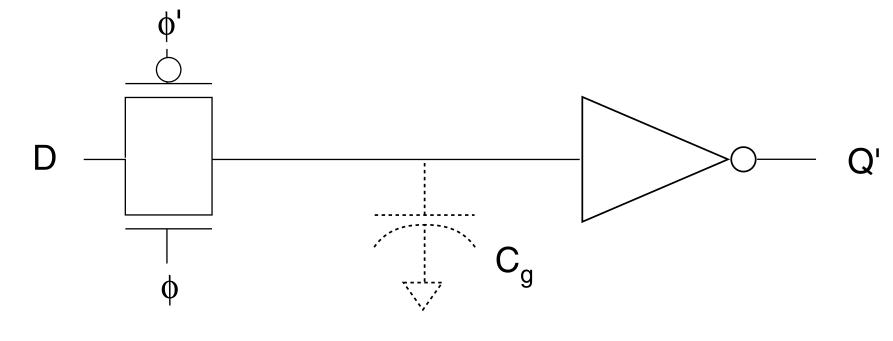
\includegraphics[width=0.7\linewidth]{Imagenes/02/02-LatchDinamica.png}
    \caption{un esquema de la latch-dinámica.}
    \label{Fig:02-LatchDinamica}
\end{figure}

El registro más simple en tecnología CMOS es el latch dinámico mostrado en la \cref{Fig:02-LatchDinamica}. Se le llama dinámico porque el valor almacenado en la memoria no se refresca mediante la fuente de alimentación, y se le llama latch porque su salida sigue a su entrada mientras está habilitado.



La entrada es D en un latch tipo D, por lo que su salida es Q’. El inversor conectado a la salida debería resultarte familiar. La capacitancia de almacenamiento se ha representado con líneas punteadas, ya que es un componente parasitario; esta capacitancia se ha denominado $C_g$ porque la mayor parte de ella proviene de las puertas de los transistores en el inversor.

El funcionamiento del latch es sencillo. Cuando el transistor de transmisión está encendido, cualquier puerta lógica conectada a la entrada D puede cargar o descargar $C_g$. A medida que el voltaje en $C_g$ cambia, Q’ sigue ese cambio de forma complementaria: cuando $C_g$ se lleva a voltajes bajos, Q’ sube a voltajes altos, y viceversa. Cuando el transistor de transmisión se abre, $C_g$ queda desconectado de cualquier puerta lógica que pudiera cambiar su valor. Por lo tanto, el valor de la salida Q’ del latch depende del voltaje del condensador de almacenamiento: si el condensador se ha descargado, la salida del latch será un 1 lógico; si el condensador se ha cargado, la salida del latch será un 0 lógico. Es importante notar que el valor de Q’ es el complemento lógico del valor presentado al latch en D; debemos tener en cuenta esta inversión al usar el latch. Para cambiar el valor almacenado en el latch, podemos cerrar el transistor de transmisión estableciendo $\phi = 1$ y $\phi’ = 0$, y luego cambiar el voltaje en $C_g$.

\begin{figure}[H] \centering
    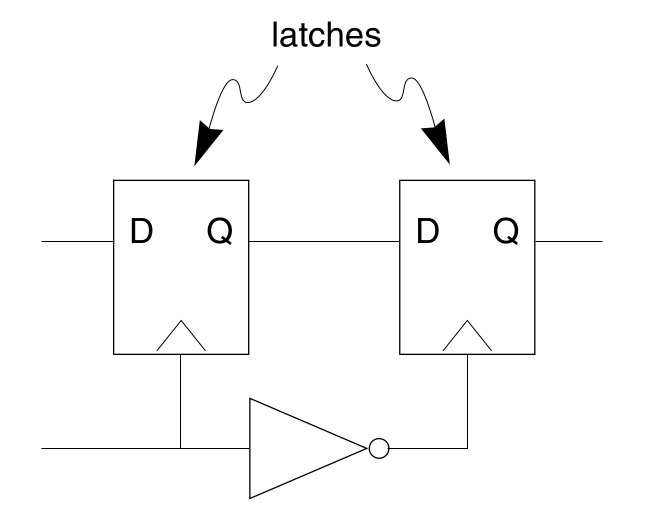
\includegraphics[width=0.6\linewidth]{Imagenes/02/02-FlipFlop.png}
    \caption{un flip-flop hecho de latches.}
    \label{Fig:02-FlipFlop}
\end{figure}

La estructura de un flip-flop activado por flanco se muestra en la \cref{Fig:02-FlipFlop}. Se construye a partir de dos latches conectados en cascada. El primer latch lee la entrada de datos cuando el reloj está en alto. Mientras tanto, el inversor interno asegura que la entrada de reloj del segundo latch esté en bajo, aislando al segundo latch de los cambios en la salida del primer latch y manteniendo estable el valor de salida del flip-flop. Después de que el reloj pasa a nivel bajo, la entrada de reloj del segundo latch queda en alto, haciéndolo transparente, pero el primer latch presenta un valor estable al segundo latch. Cuando el reloj vuelve de 0 a 1, el segundo latch guarda su valor antes de que la salida del primer latch tenga oportunidad de cambiar.

\subsection{Memoria de Acesso Aleatorio (RAM)}

La \textbf{memoria de acesso aleatorio} (RAM, \textit{Random Acess Memory}) se suele usar en FPGAs debido a que estos implementan grandes bloques de memoria. Las FPGAs usan RAM estáticas (SRAM) porque la memoria RAM dinámica comunmente se usa para \textit{bulk memory}\footnote{Bulk memory se refiere a una memoria de gran capacidad que se usa principalmente para almacenar grandes cantidades de datos, como tablas, imágenes, buffers, programas o conjuntos de datos.} requiere que el capacitor esté espacializado en estructuras que no pueden ser construidos en chips con transistores lógicos de altas capacidades. 



\subsubsection{SRAM}
Una memoria \textbf{SRAM} (\emph{Static Random-Access Memory}) es un tipo de memoria de acceso aleatorio en la que cada bit de información se almacena mediante un biestable o \textit{latches}, es decir, un circuito formado típicamente por seis transistores (en tecnología CMOS) que mantiene su estado mientras se le suministre energía. El almacenamiento de datos se realiza de manera estable gracias a la retroalimentación positiva de los biestables. Por este motivo, las SRAM ofrecen tiempos de acceso más rápidos que las DRAM.

En la \cref{Fig:02-SRAM} mostramos el núcleo principal de una SRAM. El valor se guarda en medio de los 4 transitores, que forma un par de inversores conectados en un loop. Los otros dos transitores controlan el acesso a las {celdas de memoria} \footnote{Es la unidad básica de almacenamiento en una memoria; cada celda guarda un solo bit (0 o 1)}. a través de las \textit{bit lines} (lineas de bit\footnote{Son los conductores verticales en una matriz de memoria que se usan para leer y escribir los datos de las celdas de memoria; cada bit line conecta una columna de celdas}).  Cuando select = 0, los inversores se refuerzan mutuamente para almacenar el valor. La lectura o escritura se realiza cuando la celda está seleccionada:


\begin{itemize}
    \item Para leer, las líneas bit y bit’ se precargan a $V_{DD}$ (5V) antes de que la línea de selección se active (se ponga en alto). Uno de los inversores de la celda tendrá su salida en 1 y el otro en 0; cuál de los dos está en 1 depende del valor almacenado. Por ejemplo, si la salida del inversor de la derecha es 0, la línea bit’ se descargará a $V_{SS}$ (0V) a través del transistor de bajada (pulldown) de ese inversor y la línea bit permanecerá alta. Si el valor opuesto está almacenado en la celda, la línea bit se llevará a nivel bajo mientras que bit’ permanecerá alta.
    \item Para escribir, las líneas bit y bit’ se configuran con los valores deseados, y luego se pone select en 1. El intercambio de carga (charge sharing) fuerza a los inversores a cambiar de valor, si es necesario, para almacenar el valor deseado. Las líneas de bit tienen una capacitancia mucho mayor que los inversores, por lo que la carga en las líneas de bit es suficiente para dominar al par de inversores y hacer que cambien de estado.

\end{itemize}

\begin{figure}[H] \centering
    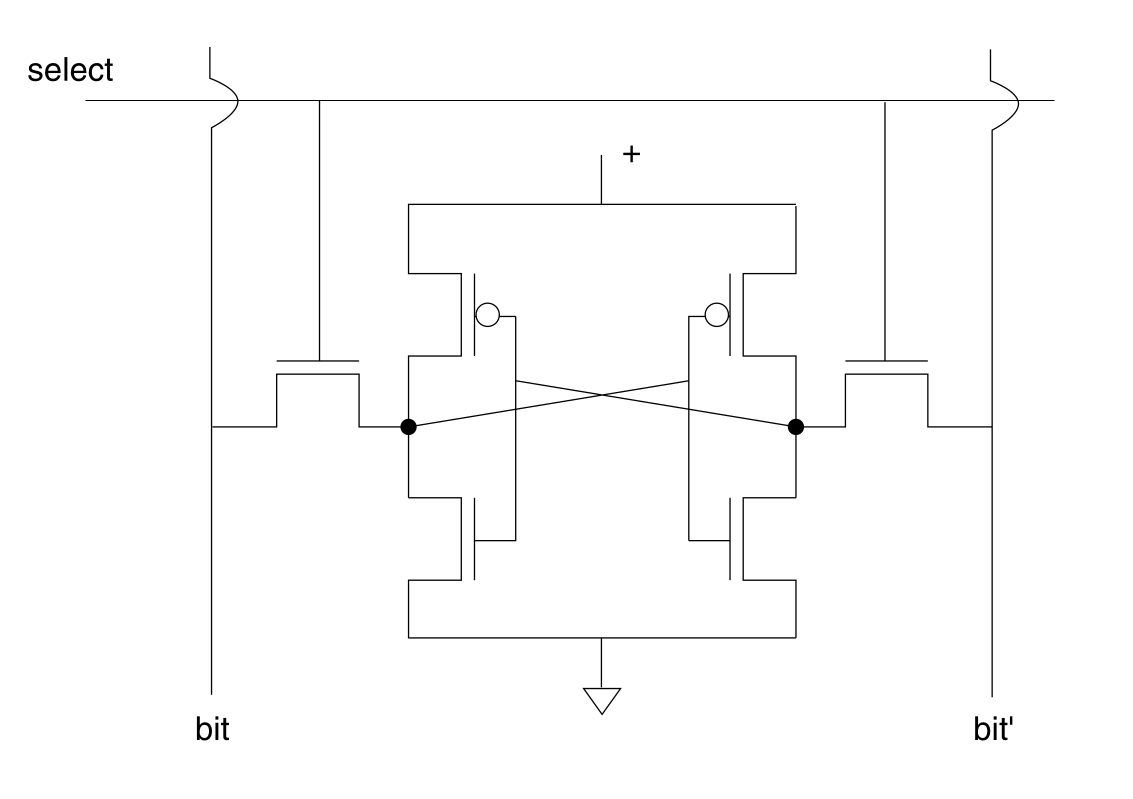
\includegraphics[width=0.6\linewidth]{Imagenes/02/02-Sram.png}
    \caption{Diseño del núcleo principal de una SRAM.}
    \label{Fig:02-SRAM}    
\end{figure}

\subsubsection{}


\chapter{Estrcuturas de sistemas FPGA}

\section{Arquitectura FPGA}

Las FPGAs están formadas por 3 tipos de elementos princiaples: 

\begin{itemize}
    \item Elementos de lógica combinacional.
    \item Interconexiones.
    \item Piones I/O (\textit{In}/\textit{Out})
\end{itemize}
\begin{figure}[H] \centering
    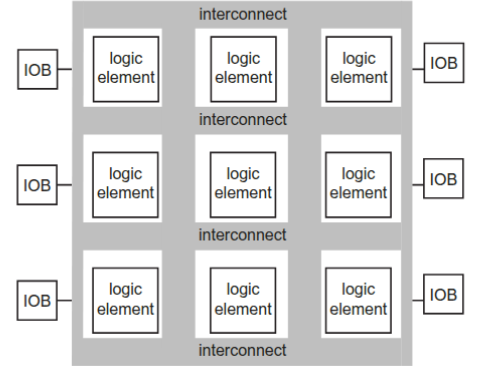
\includegraphics[width=0.6\linewidth]{Imagenes/03/03-FPGA_Fabrics.png} 
    \caption{Estructura genérica de la FPGA.}   
    \label{Fig:03-FPGA_Fabric}
\end{figure}
Estos tres elementos se combinan como puede verse en la \cref{Fig:03-FPGA_Fabric}, en los que los pines interaccionan con los elementos de lógica combinacional a través de las interconexiones. La lógica combinacional está dividida en unidades pequeñas, conocidas como \textbf{elementos de lógica} (LEs, \textit{logic elements}) o \textbf{bloques de lógica combinacional} (CLBs, \textit{combinational logic blocks}). Los LE o CLB pueden llegar a actura como las típicas puertas lógicas, claro que con na potencia mucho menor que la que podríamos encontrar en un bloque lógico combinacional encontrados en diseños grandes. Las interaconexiones se encuentran entre los elementos lógicos, y se programan (se selque tieneneccionan cuales están activas y cuales no). La interconexión suele estar organizada en canales u otras unidades. Los FPGAs normalmente ofrecen diferentes tipso de interconexiones dependiendo de la distancia entre los elementos lógicos combinacionales que tienen que conectarse. Las señales de reloj también son transportadas a través de su propia red de interconexión. Los pines I/O se llaman en general \textbf{bloques I/O} (IOBs). Estos también son programables, seleccionando si queremos que sean \textit{inputs} o \textit{ouputs}, y a veces cumplen objetivos tales como conexiones de baja potencia o alta velocidad. 

\begin{figure}[H] \centering
    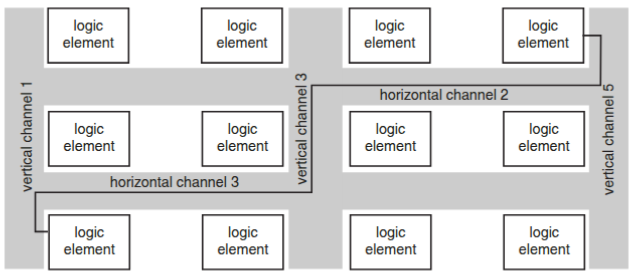
\includegraphics[width=0.6\linewidth]{Imagenes/03/03-FPGA_Interconexion.png} 
    \caption{Estructura genérica de la FPGA.}   
    \label{Fig:03-FPGA_Interconexion}
\end{figure}
Un diseñador de FPGAs debe estar dispuesto a usar diseños de conexiones preestablecidos, no como un diseñador VLSI que dibuja directamente las conexiones. El sistema de interconexión en los FPGAs suele ser uno de sus aspectos más complejos, debido a su cableado como propiedad global del diseño lógico. En la \cref{Fig:03-FPGA_Interconexion} se puede ver como sucede la interconexión entre elementos lógicos a través de un cambino complicado entre diferntes canales elegido por el diseñador.

Las conexiones entre elementos lógicos require caminos complejos debido a que los elementos lógicos LEs están dispuestos en una especie de estructura dos dimensional, por lo que las conexiones no solo son entre LEs, sino entre cables también. Los cables se organizan en tods tipos principales, los \textbf{canales cableados} y los \textbf{canales de ruta}. Los primeros corren los canales horizontales y los segundos los verticales. El diseñador es el que elige cual será usado para transportar la señal. 

Para poder permitir al diseñador lógico hacer todas las conexiones deseadas entre elementos lógicos, los canales FPGA deben estar provistos de cables de varios tamaños. Normalmente se usa la \textbf{estructura segmentada}, dado que cada cable esta formada por difernetes secciones de varias llongitudes. 

Todas las FPGAs necesitan ser programadas o configuradas. Existen tres tipos principales de FPGAs (tres tecnologías de circuitos): SRAM, \textit{antifuse} (antifusible) y \textit{flash}. No importa el tipo de circuito usado, los elementos principales de las FPGAs (lógica, interconexión, pines I/O) necesita ser configurada. Algunas de las características de interés para un diseñador que quiere usar un FPGA suele ser: 

\begin{itemize}
    \item ¿Cuánta lógica puede entrar en un FPGA? 
    \item ¿Cuantos pines I/O tengo? 
    \item ¿Cómo de rápido corre? 
\end{itemize}
Mientras que podemos determinar facilmente cuantos pines I/O tenemos, determinar la cantidad de lógica que podemos implementar y cuán rápido lo va a hacer es mucho más complicado. 



\section{FPGA basadas en SRAM}

Los FPGAs con memoria estática es uno de los más usados. 


\subsection{Elementos lógicos}

El método básico utilizado para construir un \textbf{bloque de lógica combinacional} (CLB), también llamado \textbf{elemento lógico} (LE), en un FPGA basado en SRAM es la \textbf{tabla de búsqueda} (LUT), cuyo esquema se puede ver en la \cref{Fig:03-LUT}. La tabla de búsqueda es una SRAM que se usa para implementar una tabla de verdad. Cada dirección en la SRAM representa una combinación de entradas del elemento lógico. El valor almacenado en esa dirección representa el valor de la función para esa combinación de entradas de n variables. Una función de n entradas requiere una SRAM con $2^n$ posiciones. Dado que una SRAM básica no está sincronizada con un reloj, la tabla de búsqueda (LE) opera como cualquier otra puerta lógica: a medida que cambian sus entradas, su salida cambia tras un cierto retraso.

\begin{figure}[H] \centering
    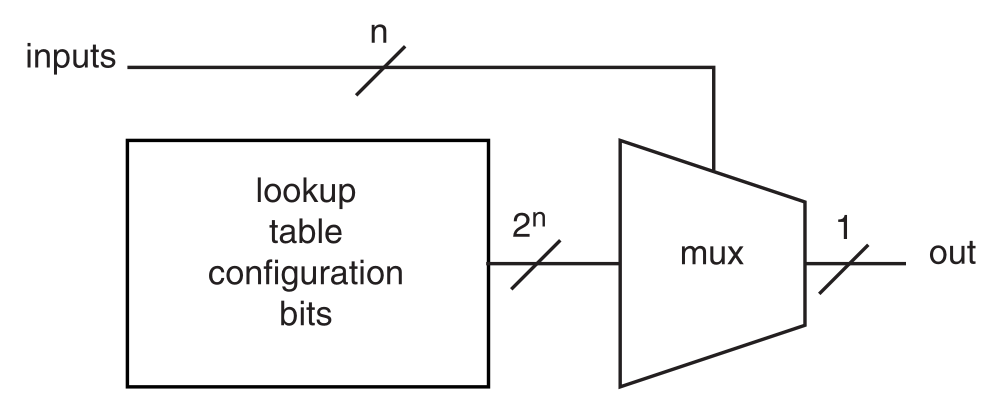
\includegraphics[width=0.6\linewidth]{Imagenes/03/03-LUT.png}
    \caption{esquema de una tabla de búsqueda (LUT).}
    \label{Fig:03-LUT}
\end{figure}

La razón por la que una función lógica de $n$ entradas necesita una SRAM con $2^n$ localizaciones es que cada combinación posible de los $n$ bits de entrada debe estar asociada a una salida determinada. Dado que cada entrada puede ser 0 o 1, el número total de combinaciones diferentes de $n$ bits es $2^n$ y, por lo tanto, para cubrir todas las posibilidades, la memoria necesita al menos $2^n$ direcciones (localizaciones). Cada dirección almacena la salida correspondiente a una combinación particular de entradas, permitiendo así implementar cualquier función booleana de $n$ entradas al usar las entradas como dirección en la memoria y leer la salida almacenada en esa dirección. Supongamos una función de 3 entradas $A$, $B$, $C$. Entonces $n=3$, y el número de localizaciones necesarias es
$$
2^3=8.
$$
Las combinaciones posibles de entrada y su dirección en la SRAM serían:

\[
\begin{array}{c c c | c}
A & B & C & \text{Dirección (binario)} \\
\hline
0 & 0 & 0 & 000 \\
0 & 0 & 1 & 001 \\
0 & 1 & 0 & 010 \\
0 & 1 & 1 & 011 \\
1 & 0 & 0 & 100 \\
1 & 0 & 1 & 101 \\
1 & 1 & 0 & 110 \\
1 & 1 & 1 & 111 \\
\end{array}
\]

Cada combinación corresponde a una localización de la SRAM: por ejemplo, si $A=0$, $B=1$, $C=0$, la combinación es 010 en binario, lo que corresponde a la dirección 2 (en decimal) de la SRAM, donde se almacena el valor de salida deseado para esa combinación.


A diferencia de una puerta lógica típica, la función representada por el LE (elemento lógico) puede cambiarse modificando los valores de los bits almacenados en la SRAM. Como resultado, un LE de n entradas puede representar $2^{2^n}$ funciones (aunque algunas de estas funciones son permutaciones entre sí). Un elemento lógico típico tiene cuatro entradas.

El retardo a través de la tabla de búsqueda (lookup table) es independiente de los bits almacenados en la SRAM, por lo que el retardo del elemento lógico es el mismo para todas las funciones. Esto significa que, por ejemplo, un LE basado en una tabla de búsqueda exhibirá el mismo retardo para una XOR de 4 entradas y para una NAND de 4 entradas. En contraste, una XOR de 4 entradas construida con lógica CMOS estática es considerablemente más lenta que una NAND de 4 entradas. Por supuesto, la puerta lógica estática es, en general, más rápida que el LE.

Los elementos lógicos generalmente contienen registros—flip-flops y latches—además de lógica combinacional. Un flip-flop o latch es pequeño comparado con el elemento de lógica combinacional (en marcado contraste con la situación en VLSI personalizado), por lo que tiene sentido añadirlo al elemento de lógica combinacional. Usar una celda separada para el elemento de memoria simplemente consumiría recursos de enrutamiento. Así los fabricantes pueden optimizar el ruteo local: el resultado de la LUT puede registrarse justo al lado, evitando que la señal viaje a bloques separados para sincronizarse, reduciendo tiempos de propagación. Además, los flip-flops permiten que el bloque lógico mantenga valores entre ciclos de reloj, posibilitando lógica secuencial. Si solo necesitas lógica combinacional, tu circuito produce salidas que dependen únicamente de sus entradas actuales, pero si quieres que tu circuito “recuerde” lo que pasó antes —es decir, que su comportamiento dependa no solo de las entradas actuales, sino también de entradas pasadas— necesitas almacenar estados (así obtenemos una \textit{lógica secuencial}). Esto se hace a través de \textit{flip-flops} y \textit{latches}.


También son posibles bloques lógicos más complejos. Por ejemplo, muchos elementos lógicos también contienen circuitería especial para la suma. Muchas FPGAs incorporan lógica especializada para sumadores dentro del elemento lógico. El componente crítico de un sumador es la cadena de acarreo (\textit{carry chain}), que puede implementarse de manera mucho más eficiente en lógica especializada que usando técnicas estándar basadas en tablas de búsqueda. Podemos ver la definción de acarreo en \cref{Sec:A-Acarreo}. 

Los ejemplos siguientes describen los elementos lógicos en dos FPGAs. Estos ejemplos ilustran tanto las similitudes entre las estructuras de FPGAs como los enfoques variados en el diseño de los elementos lógicos.


\vspace*{1em}

\begin{Ejemplo}
Ejemplo 3.1: Elementos lógicos Xlinx Spartan-II
\end{Ejemplo}

En la \cref{Fig:03-Xilinx-Spartan-II} vemos el bloque lógico combinacional Xilinx Spartan II. Una slice incluye dos celdas lógicas (LCs). La base de una celda lógica es el par de tablas de búsqueda de cuatro bits. Sus entradas son F1-F4 y G1-G4. Cada tabla de búsqueda también puede usarse como una memoria RAM síncrona de 16 bits o como un registro de desplazamiento de 16 bits. Cada \textit{slice}\footnote{Un slice es como un mini-bloque lógico que puedes programar para implementar una pequeña parte de tu diseño: una puerta lógica, un bit de un registro, una parte de un sumador, etc.}  (LUTs, flip-flops..) también contiene lógica de acarreo para cada LUT, de modo que se puedan realizar sumas. Un acarreo de entrada al slice ingresa por la entrada CIN, pasa a través de los dos bits de la cadena de acarreo, y sale por COUT. La lógica aritmética también incluye una puerta XOR. Para construir un sumador, la puerta XOR se usa para generar la suma y la LUT se usa para el cálculo del acarreo. Cada slice incluye un multiplexor que se utiliza para combinar los resultados de los dos generadores de funciones en un slice. Otro multiplexor combina las salidas de los multiplexores en los dos slices, generando un resultado para todo el CLB.

Los registros pueden configurarse como flip-flops tipo D o como latches. Cada registro tiene señales de reloj y habilitación de reloj. Cada CLB también contiene dos drivers de tres estados (conocidos como BUFTs) que pueden usarse para manejar buses internos del chip.

\begin{figure}[H] \centering
    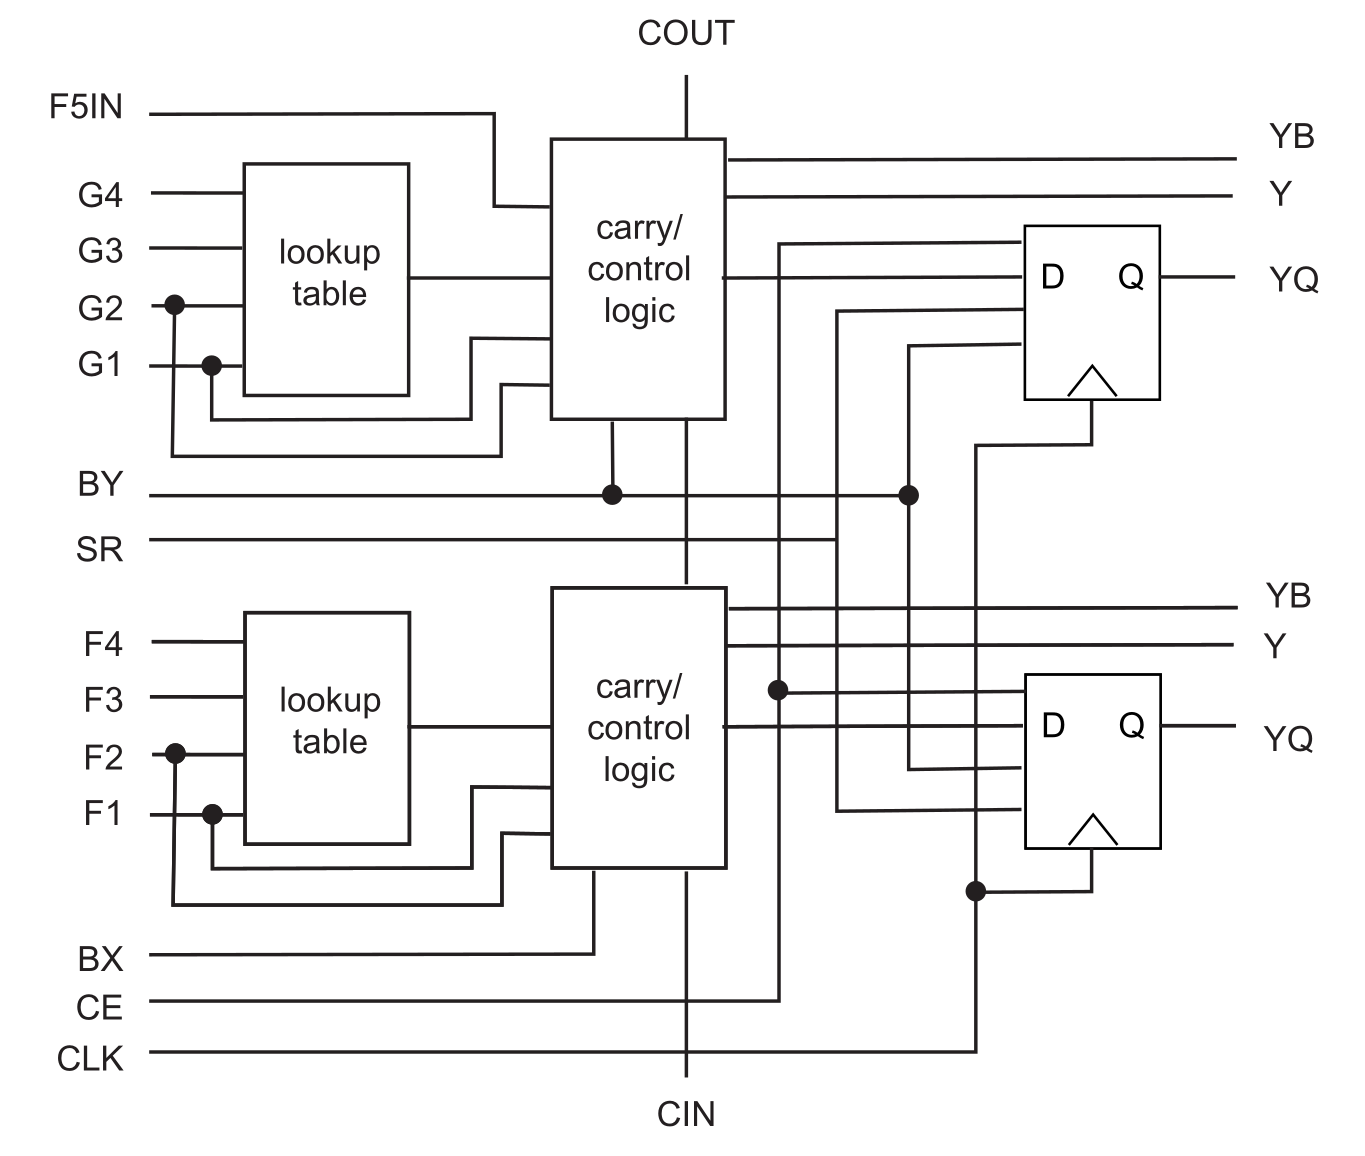
\includegraphics[width=0.6\linewidth]{Imagenes/03/03-Xilinx_Spartan_II.png}
    \caption{Elementos lógicos Xilinx Spartan II}%\cite{FPGA-WolfWayne}.}
    \label{Fig:03-Xilinx-Spartan-II}
\end{figure}

\vspace*{1em}

\begin{Ejemplo}
Ejemplo 3.2: Elementos lógicos Altera APEX II
\end{Ejemplo}


\subsection{Redes interconectadas}
\chapter{VHDL}

\section{Elementos básicos VHDL}

Un sistema digital está descrito por sus entradas, sus salidas, y la relación que existe entre ellas. En el caso de VHDL por ul sado se describe el aspecto exterior del circuito: entradas y salidas; y por otro la forma de relacionar las entradas con las salidas. El aspecto exterior, cuántos puertos es lo que denominamos \textbf{entity}. La descricpión del comportamiento del circuito es \textbf{architecture}. Toda \textit{architecture} debe estar asociada a una \textit{entity}.

Además, podemos definir bibliotecas y paquetes que vamos a usar que nos indica el tipo de puertos y operadores qeu podemos utilizar. Siempre ha de aparecer la definición de las bibliotecas y paqeutes antes de la \textit{entity}. 

\subsection{Entidad}

La entidad es la abstracción de un circuito, ya sea desde un complejo sistema electrónico o una simple puerta lógica. La entidad únicamente describe la forma externa del circuito, en ella se enumearn las entradas y las salidas del diseño. Una entidad es análoga a un símbolo esquemático en los diagramas electrónicos, el cual describe las conexiones hacia el resto del diseño. 

\begin{itemize}
    \item Define externamente al circuito o subcircuito.
    \item Nombre y número de puertos, tipos de entrada y salida. 
    \item Tienes toda la información necesaria para conectar el circuito a otros circuitos. 
\end{itemize}

\begin{lstlisting}
    entity nombre is 
        generic (cte1: tipo:= valor1; cte2: tipo = valor2: ...)
        port (entrada1,entrada2,...: in tipo;
              salida1, salida2,...: out tipo;
              puertoi: modo tipo);
    end nombre
\end{lstlisting}
Los puertos pueden ser de entrada \textbf{in} de salida \textbf{out} o de entrada-salida \textbf{inout}. Los puertos de entrada sólo se pueden leer y no se pueden modificar su valor internamente en la descripción del comportamiento interno (\textit{architecture}). 

Además se pueden generar unos valores genéricos (\textbf{generic}) que se utilizarán para declarar propiedades y constantes del circuito, independientemente de cual sea la arquitectura. A nivel de simulación, utilizaremos \textit{generic} para definir retardos de seañles y ciclos de reloj, independientemente de cual sea la atquitectura. También se podrían usar para introducir constantes utilizadas posteriormente en \textit{architecture} (como el número de registros). 

\subsection{Arquitectura}

Los pares de entidades y artquitecturas se utilizan para representar la descripción completa de un diseño. Una arquitectura describe ell funcionameinto de la entidada a la que hace referencia. Una arquitectura describe el funcioanemiento de la entidad a la que se hace refeencia, es decir, dentro de \textit{architecture} tendremos que describir el funcionamiento de la entidad utilizando las sentencias y expresiones propias de VHDL. 

\begin{itemize}
    \item Define internamente el circuito. 
    \item Señales internas, funciones, procedimientos, constantes...
    \item La descripción de la arquitectura puede ser estructural o por comportamiento. 
\end{itemize}

\begin{lstlisting}
    architecture arch_name of entity_name is 
    -- declaraciones de la arquitectura: 
    -- tipos 
    -- señales
    -- componentes

    begin 
    -- codigo de descripción
    -- instrucciones concurrentes 
    -- ecuaciones booleanas
    -- componentes
        processs (lista de sensibilidad)
        begin 
        -- codigo de descripcion
        end process
    end arch_name
\end{lstlisting}
El codigo VDHL se escribe dentro de \textit{architecture}. Cada \textit{architecture} va asociada a una \textit{entity} y se indica en la primera sentencia. A continuación, antes de \textit{begin} se finen todas las variables (señales) internas que vas a necesitar para describir el comportamietno de nuestro circuito, se definen los tipos particulares que vamos a utlizar y los componentes, otros circuitos ya definidos y compilados de los cuales conocemos su interfaz en VHDL.

El \textbf{process} es una estrucutra particular de VDHL que se reserva principalmente para contener sentencias que no tengan que tener definido su valor para todas las entradas. Esto obliga a que la estructura process almacene los valores de sus señales y pueda da lugar a circuitso secuenciales. Además, en simulación solo se ejecutan las sentencias internas a esta estrucura cuando alguna de las eñales de su lista de sensibildad carece de valor. 

\subsection{Indentificadores}

En VDHL existen tres clases de objetos por defecto: 

\begin{itemize}
    \item \texttt{\textbf{Constant.}} Los objetos de esta clase tienen un valor inicial que les es asignado de manear previa a la simulación y no puede ser modificado.   
    
    \begin{lstlisting}
        constant indentificador: tipo := valor
    \end{lstlisting}

    \item \texttt{\textbf{Variable.}} Los ibjetos de esta clase contiene un único valor que puede ser modificado durante la simulación con una sentencia de asignación. Las variables se usan como índices, o para tomar v alores que permiten modelar las componentes.  
    
    \begin{lstlisting}
        variable indentificador: tipo [:=valor]
    \end{lstlisting}

    \item \texttt{\textbf{Signal.}} Las señales representan elementos de memoria o conexiones que sí pueden ser sintetizados, dicho de otra manera, a cada objeto de nuestro codigo de VHDL que sea declarado como \textit{signal} le corresponde un cable o un elemento de memoria en nuestro circuito. Por lo tnato, su comportamiento en simulación será el esperado de ese elemento físico aunque no lo describamos explícitamente. Tienen que ser usados antes del \textit{begin} de \textit{architecture}. Los puertos de una entidad son implícitamente declarados como señales en el momento de la declaración, ya que estos representan conexiones. 

    \begin{lstlisting}
        signal indentificador: tipo
    \end{lstlisting}

    La asignacion se hace a través del operador $<=$

    \begin{lstlisting}
        nomrbe señal <= valor o expresión; 
        A <= 10
    \end{lstlisting}

\end{itemize}
Cuando se usen únicamente \textit{constant} y \textit{signal} no se observarán efectos perversos. Además, el código obtenido podrá ser sintetizado en cualquier herramient. Por eso mismo en este manual a partir de este momento cuando nos refiramos a una señal nos referiremos a un objeto \textit{signal} y solo trabajaremos con estos. 

Existen varios tipos de objetos: 

\begin{itemize}
    \item \textbf{std\_logic}. Tipo predefinido en el estandar IEE 1164. Este tipo reprsenta una lógica multivaluada de 9 valores. Tenemos el 0 y 1 lógicos, así como Z (alta impedancia), X (desconocido), U (sin inicializar).
    \item  \textbf{std\_logic}(rango). Representa un vector de elementos \textit{std\_logic}. Para un vector de N elementos el rnago será \textit{N-1 dowto 0}. 
\end{itemize}
Podemos escribir todas las asignaciones del código ya sean operaciones sencillas, opoeraciones aritmeticológicas y comparaciones utilizando \textit{std\_logic\_vector}, sin complicar el código y ayudando a su interación en XILINX. 

\begin{itemize}
    \item \texttt{Alias.} Los alias no son un tipo de indentificador, es una manera de nombrar a un elemento ya existente. El alias nos ayuda a mejorar la legilidad del código que estamos implementando, admeás nos puede ayudar a simplificar el manejo del identificador. 
    \begin{lstlisting}
        alias nombre: tipo is indentificador(rango);
    \end{lstlisting}
\end{itemize}
Un ejemplo del uso de alias: 

\begin{lstlisting}
    signal CTRL: std_logic_vector (7 downto 0); 
    alias c_mux_8a1: std_logic_vector (2 dowto 0) is CTRL (7 downto 5)
    alias load_ref1: std_logic is CTRL(4)
\end{lstlisting}

\subsection{Operadadores}

Un operador nos permite constuir diferentes signos de expreisones mediante los cuales podemos calcular datos utilizando diferentes señales. 


\section{Estructura básica de un archivo fuente en VHDL}

Como hemos dicho, los modelos VDHL están formados por dos partes: la entidad y la arquitectura. En esta última es donde se escriben las setencias que describen el comportamiento del circuito, a este modelo de programación se suele denominar \textit{behavioral}. El esquema básico será: 

\begin{lstlisting}
    architecture circuito of nombre es 
    -- señales
    begin 
    -- sentencias concurrentes
    process (lista de sensibilidad)
    begin 
    -- sentencias secuenciales
    -- setencias condicionales
    end process
    end architecture circuito; 
\end{lstlisting}
Dentro de la arquitectura se encuentra: 
\begin{enumerate}
    \item Tipos y sñales intermedias necesarias para la descripción del comportamiento. 
    \item Setencias de asingación que deben realizarse siempre así como secuencias concurrentes.
    \item Uno o varios \textit{process} qeu tienen lugar en su interior sentencias condicionales y/o asignaciones a señales qeu dan lugar a hardware secuencial. 
\end{enumerate}

\subsection{Sentencias concurrentes}

Son sentencias condicionales que tienen al menos un valor por defecto para cuando no se cumplen niguna de las condicoines. Podría utilizarse una setencia común con un if y un else, los desarrolladores de VDHL prefirieron históricamente otras setencias.

\begin{itemize}
    \item 
La sentencia \texttt{when-else} evalúa condiciones de forma jerárquica. Es similar a una cascada de \texttt{if-else}. Ejemplos: 


\begin{lstlisting}[caption={Ejemplo de \texttt{when-else}}]
    Y <= "00" when "A=B" else
         "01" when "A<B" else
         "10" when "10",
         "11" when others;
\end{lstlisting}

    \item 
La sentencia \texttt{with-select-when} selecciona un valor de salida en función de una expresión y múltiples valores constantes. Ejemplos: 

\begin{lstlisting}[caption={Ejemplo de \texttt{with-select-when}}]
with entrada select
    salida <= "00" when "001",
         "01" when "010",
         "10" when "100",
         "11" when others;
\end{lstlisting}


\end{itemize}
El buen programador de VHDL debe acostrumbrarse a utilizar estas setnecias ya que le quitará muchos problemas que aparezcan: 
\begin{itemize}
    \item \texttt{when-else} es útil para condiciones booleanas.
    \item \texttt{with-select-when} es ideal para valores discretos (como multiplexores).
\end{itemize}

\subsection{Sentencias condicionales}
El programa VHDL permite utilizar otro tipo de setencias condicionales más parecidas a los leguajes de programción modernos. Todas estas setencias tienen que ir obligatoriamente en un \textit{processs}. Las mas comunes son:  

\begin{itemize}
    \item La sentencia \texttt{if-then-else} constituye de: 
    \begin{lstlisting}
    process (lista de sensibilidad)
    begin
    if condición then 
    -- asignaciones 
    elsif otra_condicioón then
    -- asignaciones 
    else 
    -- asignaciones 
    end if;
    end process;
    \end{lstlisting}
    Las sentencias if-else deben, en general, acabar con un else. 
    \item La sentencia \texttt{case-when} es: 
    \begin{lstlisting}
    process (lista de sensibilidad)
    begin
    cas señal_condición is 
        when valor_condicion_1 => 
        -- asignaciones
        ...
        when valor_condición_n =>
        -- asignaciones 
        when others ->
        -- asiginaciones
    end case: 
    end process;
    \end{lstlisting}
    Es necesario que aparezca \textit{when others}.   
    \item La sentencia \texttt{for-loop} es: 
    \begin{lstlisting}
    process (lista de sensibilidad)
    begin 
    for loop_var in range loop
        -- asignaciones
    end loop;
    end process;
    \end{lstlisting}
    Para el for, \textit{range} puede ser 0 to N o N downto 0.
    \item La sentencia \texttt{while-loop} es: 
    \begin{lstlisting}
    process (lista de sensibilidad)
    begin
    while condición loop    
        -- asignaciones
    end loop;
    end process;
    \end{lstlisting}
    El bucle for está soportado si elrango del índice es estático (\textit{0 to N}) y el cuerpo contiene sentencias \textit{wait}. 
\end{itemize}


\subsection{Setencias process}

VHDL presenta una estructura particular denominada \textit{process} que define los límites de un dominio que se ejecutará (simulará) si y sólo si alguna de las señales de su lista de sensibilidad se ha modificado en el anterior paso de simulación. Un process tiene la siguiente estructura: 

\begin{lstlisting}
    process (lista_de_sensibildad)
    -- asingacion de variables
    -- opcional no recomendable
    begin 
    -- Setencias condicionales
    -- Asingaciones 
    end process; 
\end{lstlisting}
Es una de las sentencias mas utilizadas ya que tanto las setencias condicionales como la descricpión del Hard-Ware secuencia se realiza dentro de él. Veamos algunas de las propiedades: 

\begin{itemize}
    \item \textbf{Propiedad I}: solo se ejecutan las intrucciones internas en el instante 0 de simulación y cuando varía alguna de las señales de su lista de sensibilidad. Para solucionar el posible problema lo que necesitamos es incluir al menos todas las señales que se lean dentro del \textit{process}.
    
    \vspace*{1em}
    
\begin{minipage}{0.47\linewidth} \centering
    \begin{lstlisting}
    process (A)
    begin
        if B='1' then
            C <= A;
        end if;
    end process;
    \end{lstlisting}
\end{minipage}\hfill
\begin{minipage}{0.47\linewidth} \centering
    \begin{tabular}{|c|c|c|c|}
    \hline
    \textbf{t} & \textbf{0 ns} & \textbf{5 ns} & \textbf{10 ns} \\
    \hline
    \textbf{A} & 0 & 0 & 1 \\
    \hline
    \textbf{B} & 0 & 1 & 1 \\
    \hline
    \textbf{C} & U & U & 1 \\
    \hline
    \end{tabular}
\end{minipage}
%\end{itemize}
%\begin{itemize}
    
\vspace*{-0.5em}
    
    Como podemos ver no se asigna a C un valor hasta que en el instante 10 ns, pese a que B  cambió en el instante 5 ns, esto es, deibido a que no se entra dentro del process hasta que A no varía (instante 10 ns). Sin embargo a nivel Hardware esperaríamos que C tomase el valor de A en el mismo instante en el que B cambia a 1 (en 5 ns). La solución sería: 
    
\vspace*{1em}
    

\begin{minipage}{0.47\linewidth} \centering
    \begin{lstlisting}
    process (A,B)
    begin
        if B='1' then
            C <= A;
        end if;
    end process;
    \end{lstlisting}
\end{minipage}\hfill
\begin{minipage}{0.47\linewidth} \centering
    \begin{tabular}{|c|c|c|c|}
    \hline
    \textbf{t} & \textbf{0 ns} & \textbf{5 ns} & \textbf{10 ns} \\
    \hline
    \textbf{A} & 0 & 0 & 1 \\
    \hline
    \textbf{B} & 0 & 1 & 1 \\
    \hline
    \textbf{C} & U & 1 & 1 \\
    \hline
    \end{tabular}
\end{minipage}

    \item \textbf{Propiedad II}: las asignaciones a señales que se realizan dentro de un process tienen memoria. Si en un paso de simulación se entra dentro del \textit{process} y debido a las sentencias internas se modficia el valor de la señal C, y en otro paso de simulación posterior se entra dentro del \textit{process} pero no se modifica C, la señal C cosnervará el valor asignado con anterioridad. 
    \item \textbf{Propiedad III}: dentro de un \textit{process} todas las intrucciones se ejecutan en paralelo, igual que ocurre con las intrucciones qeu se encuentran fuera de los process. Sin embargo si dentro del \textit{process} se asigna valor a una señal en dos sitios diferentes, el resultado será aquel de la última asingación, exactamente igual qeu en los leguajes de programación. Siempre hay qeu comprobar qeu no estamos asignado el valor a unsa señal en dos sitios diferentes del \textit{process} (si puede hacerse en dos ramas diferentes del mismo \textit{if}).
    \item \textbf{Propiedad IV}: los \textit{process} se ejecutan en paralelo. Siempre hay qeu comprobar que no se modidfica la misma señal en dos \textit{process} diferentes, en caso de que esto ocurra habrá que fusionar los  \textit{process}. 
    \item \textbf{Propiedad V}: los valores de las señales que se modfiican internamente en los \textit{process} no se actualizan hasta que no se ha ejectuado el \textit{process} completo.
\end{itemize}

\subsection{Descripción estructural}

Esta descripción utiliza para la creación de la arquitectura de la entidad entidades descritas y compiladas previamente, de manera en VHDL podemos aprovechar diseños ya realizados  o realizar diseños sabiendo qeu se utilizarán otros más complicados. Así se ahorra trabajo al diseñador-programador. 

Se declaran los componentes qeu se van a utilizar 

\section{Simulación en VHDL}

VHDL realiza la simulación siguiendl a ténica de \textbf{simulación por eventos discretos} (\textit{Discrete Event Time Model}). Esta es una ténica que permite avanzar e ne ltiempo a intervalos variables, en función de la planificación de ocurrencia de eventos (cambio de valor de alguna señal). Esto significa que no se simula el comportamiento del circuito pico-segundo a pico-segundo, si no desde qeu ocurre un evento hasta el siguiente, donde puede pasar un pico-sigundo o varios segundos. Durante el intervalo de itempo en el uqe nose produce ningún evento, se mantiene el valor de todas las señales. 

\subsection{Sentencias de simulación}

VDHL presenta una sentencia específica, WAIT, que detiene la ejecución del código hasta qeu se cumpla la condición. La setencia \textit{wait} debe aparecer obligatoriamente en el \textit{process} no tiene lista de sensibilidad. Además en muchos tutoriales se utliza para generar hardware secuencial. 

\begin{itemize}
    \item \texttt{wait on lista\_de\_señales}: no se ejecutan las intrucciones posteriores hasta que no se modifique alguna de las señales de la lista. 
    \item \texttt{wait for tiempo}: no se ejecutan intrudcciones posteriores hasta que no pase el tiempo indicado desde que se llegó a la instrucción \textit{wait}.
    \item \texttt{wait ultil condicion}: no se ejecutan las intrucciones posteirores hasta que no se cumpla la condición. 
\end{itemize}

\section{Descripción de Lógica Secuencial}

Una de las propiedas más importantesdel \textit{process} es la capacidad de la estructura para almacenar los valores de las señales que se asignan en su interior di surante el paso de simulación no se entra dentro del process o no se relaiza ninguna asignación a esta señal. Debido a esta característica se utlizarán los process para generar hardware secuencial. 

\subsection{Hardware secuencial}

Para la descripción de los biestables (latches) y registros utilizaremos \textit{process} en los que la señal de reloj CLK (clk) actúe por flanco conjuntamente con un \textit{if} sin rama \textit{else}.

\begin{lstlisting}
    if (CLK'event and CLK='1') then ...
\end{lstlisting}
Así pues si se quiere representar un bietable deberíamos añadir el siguietne process: 

\begin{lstlisting}
    entity Biestable_D is 
        port (d,clk: in std_logic; q: out std_logic);
    end Biestable_D;

    architecture ARCH of Biestable_D is
    begin
        process (clk,d)
        begin
            if (clk'event and clk='1') then q<=d;
            end if
        end processs
    end ARCH;
\end{lstlisting}

\subsection{Contadores}

\chapter{Vivado y VHDL}

En esta sección presentaremos los proyectos que vayamos haciendo. 

\section{Proyecto: calculadora binaria.}




\appendix

\chapter{Definciones básicas}

\section{Acarreo} \label{Sec:A-Acarreo}

En general, el acarreo está ligado a todo circuito o algoritmo que requiera propagación de valores que exceden la capacidad de una posición binaria, por lo que es fundamental para la aritmética digital y el diseño de ALUs, sumadores, procesadores y sistemas embebidos.

Los \textbf{bits de acarreo} son los bits que se generan y se propagan entre etapas sucesivas cuando se suman números binarios. Se llaman así porque ``transportan'' el exceso cuando la suma de dos bits en una posición supera la capacidad de esa posición (es decir, cuando la suma da un resultado mayor que 1 en binario).

Por ejemplo, al sumar dos bits \(A_i\) y \(B_i\) en la posición \(i\) junto con un acarreo de entrada \(C_i\), el resultado del bit de suma es

\[
S_i = A_i \oplus B_i \oplus C_i,
\]

y el bit de acarreo de salida (hacia la siguiente posición más significativa) es

\[
C_{i+1} = (A_i \cdot B_i) + (A_i \cdot C_i) + (B_i \cdot C_i),
\]

donde \(\oplus\) representa la operación XOR, \(\cdot\) es la operación AND, y \(+\) es la operación OR en lógica booleana. Cuando se suman \(1 + 1\) en binario, se obtiene \(10\): el 0 es el bit de suma \(S_i\) y el 1 es el bit de acarreo \(C_{i+1}\) que debe sumarse a la siguiente posición más significativa. Los bits de acarreo aseguran que la suma sea correcta, de forma similar a como se ``lleva'' una unidad a la siguiente columna al sumar en el sistema decimal, por ejemplo al sumar 9 + 5. En un sumador binario de varios bits, estos bits de acarreo forman la \textbf{cadena de acarreo}, ya que cada etapa depende del acarreo generado en la etapa anterior.

La \textbf{cadena de acarreo} (en inglés, carry chain) es un elemento fundamental en los sumadores digitales. Es la secuencia de propagación de los bits de acarreo de una etapa de suma a la siguiente cuando se suman dos números binarios. En un sumador, cada bit de la suma depende de los bits de entrada y del acarreo que llega de la posición anterior: si el bit menos significativo genera un acarreo, este debe sumarse con el siguiente bit más significativo, y así sucesivamente.

En un sumador de varios bits (por ejemplo, un sumador de 4 bits), este proceso crea una cadena de acarreos que se propaga desde el bit menos significativo hasta el más significativo. Este retardo de propagación del acarreo es un factor crítico que limita la velocidad de los sumadores implementados como sumadores en serie, porque el acarreo debe recorrer cada bit antes de que el resultado final sea estable.

Por eso se diseñan sumadores más rápidos como el sumador de acarreo anticipado (carry lookahead adder) o el sumador de bloques, que intentan predecir los acarreos sin esperar a que la cadena de acarreo se propague completamente, reduciendo así el retardo total.

El concepto aparece de forma central en la aritmética digital y es clave en el diseño de ALUs (unidades aritmético-lógicas) y procesadores, porque limita el tiempo de operación de sumas, restas y otras operaciones que dependen del acarreo.

\nocite{*}
\newpage
\addcontentsline{toc}{section}{Referencias}
\printbibliography



\end{document}